% Chapter Template

\chapter{Methodology} % Main chapter title

\label{Methodology} % Change X to a consecutive number; for referencing this chapter elsewhere, use \ref{ChapterX}

This chapter provides a detailed overview of the implementation and evaluation approach used in our investigation into the impact of task-incremental continual learning using parameter-efficient methods on the retention of the innate capabilities of a pretrained model and subsequently learned tasks. In Section \ref{ResearchApproach}, we describe our research approach and the rationale behind our methodological choices. Section \ref{Data} explains in detail %, we describe 
the datasets used for training and evaluating our model and cover the data preparation and preprocessing methods used. Section \ref{Implementation} discusses the implementation pipeline and the mitigation approach used.
%----------------------------------------------------------------------------------------
%	SECTION 1
%----------------------------------------------------------------------------------------
\section{Research Approach} \label{ResearchApproach}
Our research objective focused on task-incremental learning and aimed to investigate the impact of catastrophic forgetting in training a pre-trained model on a sequence of distinct tasks. In this context, a task is a specific set of learning objectives and capabilities that the model needs to develop. Each task is characterized by a unique data distribution and distinct capabilities. Some examples include summarization, Python unit-test generation, and classification. We chose to focus on task-incremental learning for the following reasons:
\begin{itemize}
    \item It allowed us to study and measure how learning a new task affects the model’s pre-trained capabilities and its performance on previously learned tasks. 
    By comparing the performance before and after learning a new task, it allowed us to observe when and how forgetting occurs and measure the effect of catastrophic forgetting on task performance.
    \item It enabled us to identify which tasks were more prone to cause forgetting of model’s pretrained and learned task capabilities, and check if the order in which tasks appear influences forgetting.
    \item It facilitated the evaluation of the effectiveness of methods aimed at mitigating catastrophic forgetting across a range of different tasks.
\end{itemize}
For the implementation of task-incremental learning, we looked at two specific use cases: \textbf{Code Generation} and \textbf{Natural Language Generation}. For each of these use cases, we identified three distinct tasks, allowing us to evaluate the model’s ability to learn and retain diverse skills. The selection of the tasks was guided by the following considerations:
\begin{itemize}
    \item It was important to ensure that the selected tasks had sufficiently different data distributions to avoid overlap and redundancy.
    \item It was important to take the available computational resources and time limitations into consideration to ensure that the training and evaluation could be conducted within the given resource constraints.
    \item Availability of good datasets relevant to the use case and our research objectives.
\end{itemize}
Our approach involved sequentially fine-tuning a pre-trained large language model on the selected tasks. Our objective was to have a single model with the capability to perform several tasks. Thus, our process pipeline implemented task-incremental continual instruction fine-tuning using sequential training and merging of LoRA adapters. The choice of instruction fine-tuning was motivated by research showing the effectiveness of using instructions in improving model generalization to unseen tasks \cite{chung2024scaling}.

\begin{figure}[h]
    \centering
    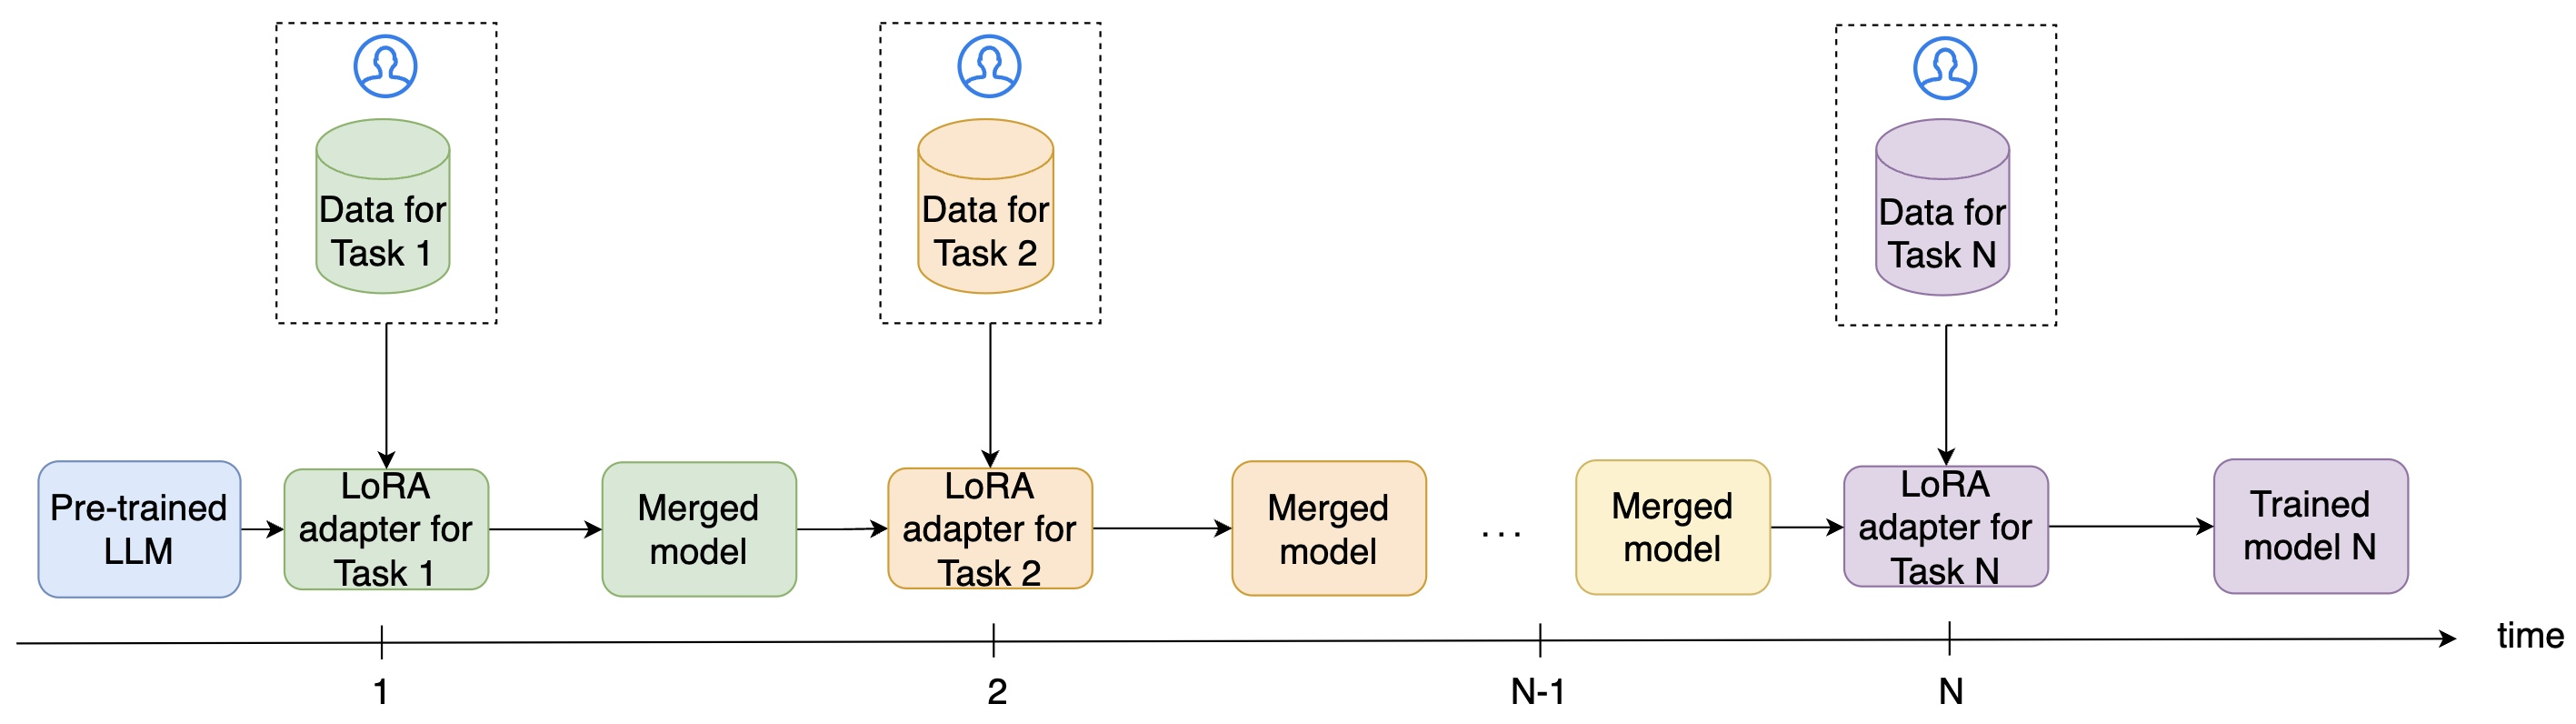
\includegraphics[width=1\textwidth]{Figures/methodology/process_pipeline.jpeg} % Replace with your image path
    \caption{Sequential Fine-tuning of LoRA adapters.}
    \label{fig:Sequential Fine-tuning of LoRA adapters}
\end{figure}


We used decoder-based causal models to study the effects of task-incremental learning on the pre-trained capabilities of the model. The models selected for each use case are listed as follows: 

\begin{table}[h]
\centering
\caption{Models selected for each use case.}
\begin{tabular}{| m{7cm} | m{6cm} |}
\hline
\textbf{Use Case} & \textbf{Model} \\
\hline
Code Generation use case & DeepSeek-Coder-6.7B-Instruct \\
\hline
Natural Language Generation use case & Meta-Llama-3-8B-Instruct \\
\hline
\end{tabular}
\end{table}

The models were selected based on their suitability to the use case tasks. DeepSeek-Coder \cite{guo2024deepseek} is specifically trained on code data, which makes it well-suited for code generation tasks. Llama models \cite{touvron2023llama} have a strong performance on a range of natural language tasks, making them apt for generic language generation tasks. The model sizes were chosen to ensure a balance between model capability and computational feasibility.

Our research objective also focused on investigating the impact of memory replay-based mitigation methods on forgetting and task-retention capability of the model. To do this, we implemented baseline comparisons of task-incremental learning without replay to analyze the impact of the mitigation approach. Our implementation also incorporated an evaluation setup with different benchmarks and task-specific performance measures. This evaluation step was performed before and after each fine-tune to compare and measure the impact of the training on the model's original capabilities and previously learned tasks.

%----------------------------------------------------------------------------------------
%	SECTION 2
%----------------------------------------------------------------------------------------
\section{Data} \label{Data}
For our task-incremental learning setup, we selected datasets that aligned with the tasks we selected for each use case. We selected three datasets for code generation use case and three datasets for natural language generation use case.

%-----------------------------------
%	SUBSECTION 1
%-----------------------------------
\subsection{Data Description} \label{Data Description}
\subsubsection{Code Generation Use Case} \label{Code Generation Use Case}
The Code Generation use case included tasks that were associated with developing a model’s capability to generate code or perform code completion based on the provided input or context. 
The tasks selected for the Code Generation use case were:
\begin{itemize}
\item \textbf{Code generation in C++.} This task involved training the model to generate code in C++ based on the provided instruction. The dataset used for this task contained code samples for function, macro, variable, and method declarations written in C and C++ from a specific repo.
\item \textbf{Unit Test generation in C++.}This task involved training the model to generate unit tests for functions written in C++. The dataset for this task contained samples with unit tests and their associated target functions from the same repo used in the C++ code generation task.
\item \textbf{Manifest (Kubernetes configuration) generation.}This task involved developing the model’s capability to generate YAML configuration files for Kubernetes deployments. The manifest generation dataset contained samples of configuration files with HELM charts and values for Kubernetes pods and service deployments.
\end{itemize}
The data sets for the Code Generation use case are private company datasets. Thus, only the results and observations from the experiments with the datasets are included in this report. 

\subsubsection{Natural Language Generation Use Case} \label{Natural Language Generation Use Case}
The Natural Language Generation use case included tasks that involved generating meaningful text based on the provided structured data. These include downstream tasks such as summarization, machine translation, and dialogue generation. 
The tasks selected for the natural language generation use case are:
\begin{itemize}
\item \textbf{Question Answering.}This task involved training the model to answer questions based on the provided input context or knowledge base. We used the ScienceQA dataset for the question answering task. ScienceQA \cite{lu2022learn} is a benchmark dataset consisting of 21,208 multimodal multiple-choice questions collected from elementary and high school Science curriculum. The questions in the dataset cover a wide range of topics from three subjects: natural science, language science, and social science. We used the subset of the ScienceQA dataset used in the TRACE benchmark \cite{wang2023trace}. This subset excludes examples with multimodal contexts. 

\item \textbf{Summarization.} The summarization task aimed to train the model to extract important information from provided input text or documents and generate concise and meaningful summaries. The dataset used for the summarization task was the MeetingBank dataset. The Meeting Bank dataset \cite{hu2023meetingbank} is a domain-specific benchmark dataset for abstractive summarization with annotations from 1366 US city council meetings.

\item \textbf{Mathematical Reasoning.}This task involved training the model to develop reasoning capabilities to solve challenging mathematical problems. With this task, we taught the model to generate step-by-step solutions with explanation for common sense and domain-specific numeric reasoning problems. The dataset used for the mathematical reasoning task was the NumGLUE dataset. NumGLUE \cite{mishra2022numglue} is a multi-task benchmark dataset focused on evaluation of a model’s performance on tasks that require arithmetic understanding. Similar to \cite{wang2023trace}, we used the first two task sub-sets of the NumGLUE dataset focused on arithmetic reasoning.
\end{itemize}

%-----------------------------------
%	SUBSECTION 2
%-----------------------------------
\subsection{Data Preparation} \label{data_preparation}
An important challenge in attaining a high-quality instruction fine-tuned model is the preparation of a high-quality instruction dataset. For this, we applied the following pre-processing and preparation steps:

%-----------------------------------
%	SUBSECTION 3
%-----------------------------------
\subsubsection{Instruction Pair Preparation}
Fine-tuning language models on data samples phrased as instructions has been shown to improve model performance and generalization to unseen tasks \cite{chung2024scaling}. The instruction fine-tuning method required the preparation of datasets with instruction and response pairs. The datasets selected for each task were not in an instruction-response pair format. Thus, a task-specific instruction needed to be created for each sample in the dataset.

The instruction pair preparation process for the code generation task was done by extracting important details from the code samples and using the details to prepare targeted instructions for the samples. For unit test generation, the same static instruction was used for all samples, since it would include the target function as input in the final generated prompt. For manifest generation task, we extracted the important variables from the manifest files and prepared targeted instructions using the extracted information.

The instructions used for the natural language generation task were either the same or modified versions of the instructions used in the datasets from the TRACE benchmark \cite{wang2023trace}. The instructions used are shown in Table \ref{tab:tasks}.

\begin{table}[H] 
    \centering
    \caption{Instructions for Natural Language Generation tasks.}
    \begin{tabular}{| m{4cm} | m{9cm} |}
    \hline
    \textbf{Task} & \textbf{Instruction} \\
    \hline
    Question Answering & Choose an answer for the following question and give your reasons. \\
     & Question: ['question'] \\
     & Choices: ['choices'] \\
     & Answer: \\
     & Your response MUST start with the letter corresponding to the correct option. \\
    \hline
    Summarization & Write a summary of the following meeting transcripts. \\
     & Meeting transcripts: ['content'] \\
    \hline
    Math & Solve the following math problem. \\
     & Question: ['question'] \\
     & Let’s think step by step. At the end, you MUST write only the final answer after '\#\#\#\#'. \\
    \hline
    \end{tabular}
    \label{tab:tasks}
\end{table}

%-----------------------------------
%	SUBSECTION 4
%-----------------------------------

\subsubsection{Prompt format}
It was important to use the prompt instruction template of the model being used to properly utilize the model. For code generation tasks, we used the prompt instruction template provided by DeepSeek.

\paragraph{DeepSeek Prompt Instruction Template} \label{DeepSeekPrompt}
\begin{lstlisting}
You are an AI programming assistant, utilizing the DeepSeek Coder 
model, developed by DeepSeek Company, and you only answer questions 
related to computer science. For politically sensitive questions, 
security and privacy issues, and other non-computer science 
questions, you will refuse to answer.
### Instruction:
['instruction']
### Input:
['input']
### Response:
['answer']
<|EOT|>
\end{lstlisting}

\paragraph{Llama3 Prompt Instruction Template} \label{Llama3Prompt}
For natural language generation tasks, we used the prompt instruction template used by Llama3.
\begin{lstlisting}
<|start_header_id|>You are a helpful AI assistant. Provide concise 
answers, focusing on the key information needed.<|end_header_id|>{{ 
system_prompt }}<|eot_id|>
<|start_header_id|>user<|end_header_id|>{{ input }}<|eot_id|>
<|start_header_id|>assistant<|end_header_id|>{{ output }}<|eot_id|>
\end{lstlisting}

%-----------------------------------
%	SUBSECTION 5
%-----------------------------------
\subsubsection{Context-Length Based Filtering}
The context length used for the generation was limited to 8K (8192) for the experiments. It was important to retain only samples that fit within the context-length limitation to ensure that the generations would always yield a usable output. Thus, a step to filter out samples that would exceed the set limit was applied to all the datasets. This was done with the following steps:
\begin{itemize}
\item The final prompt was prepared using the prompt format with the instruction, input (if necessary), and output for each data sample.
\item The model tokenizer was used to get the tokens for the final prompt.
\item The length of the tokens was computed.
\item The samples whose token length was greater than 7K (7168) were filtered out. We used 7K as the threshold since the maximum new tokens for the generations in the evaluation process is set to 1K (1024).
\end{itemize}

%-----------------------------------
%	SUBSECTION 6
%-----------------------------------
\subsubsection{Stratified sampling}
We limited the size for each task dataset to 5000 as a maximum value to allow for faster experimentation and to ensure that the fine-tuning and evaluation can be carried out with the computational resources available to us. This helped to reduce our training time and lowered our resource requirements. However, it was important for us to ensure that the sampled dataset still maintained the distribution and complexity of the original full dataset. We used stratified sampling to ensure that the proportional representation of the different categories in the original dataset was retained.

%-----------------------------------
%	SUBSECTION 7
%-----------------------------------
\subsubsection{Synthetic Data Generation} \label{Synthetic Data Generation}
For the math task, each sample in the NumGLUE dataset contained the question, the prepared instruction, and the final answer. However, the instruction asks the model to perform reasoning steps to get to the final answer. Since we did not have answers with the reasoning steps, we used an LLM to generate answers with the reasoning steps using the same instruction. We used GPT-4 to generate the answers. The generated answers were manually verified for correctness by checking them against the original final answers in the dataset. The samples where the generated answers did not match the original answers in the dataset were filtered out.

We also used LLM-based synthetic data generation to prepare datasets that would resemble the model's original training data. This was necessary because the original datasets that were used to train the models have not been released. These synthetically generated datasets would then be used to help preserve the instruct model capabilities, by integrating the step to include data samples in the replay buffer as part of the mitigation method against catastrophic forgetting. This approach would enable to maintain the model's innate capabilities throughout the continual learning process \cite{guo2024efficient}. The process for the preparation of the dataset for the code generation and natural language generation use cases is shown in Figure \ref{fig:SyntheticDataGen}.

\begin{figure}[h]
    \centering
    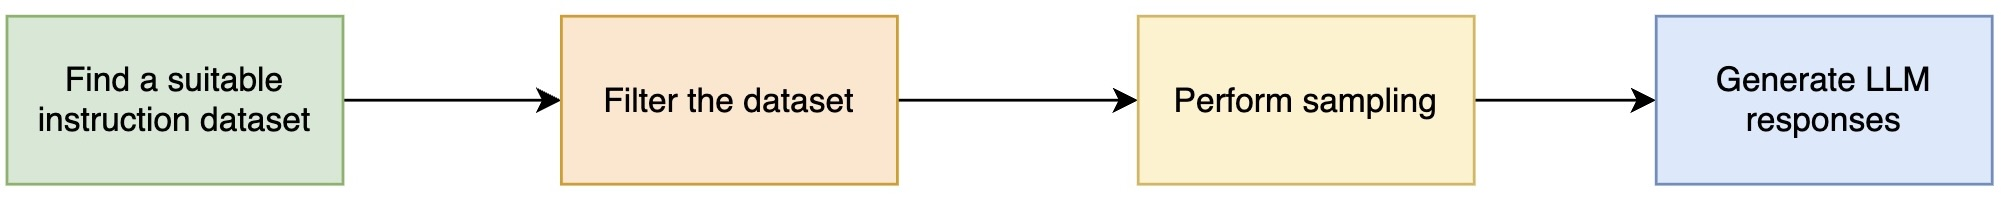
\includegraphics[width=1\textwidth]{Figures/methodology/synthetic_data_gen.jpeg} % Replace with your image path
    \caption{Synthetic Data Generation process.}
    \label{fig:SyntheticDataGen}
\end{figure}

The steps followed for preparation of the dataset for the code generation use case were as follows:
\begin{enumerate}
\item An instruction dataset that resembles the training data for the model and was published after the model release date to avoid data contamination was used. The \href{https://huggingface.co/datasets/nickrosh/Evol-Instruct-Code-80k-v1}{Evol-Instruct-Code-80k-v1} dataset was used for the code generation use case.
\item Filtering was performed to keep only the relevant samples. The code dataset was filtered to keep samples with Python, Java, and C++ code.
\item Stratified sampling was performed to reduce the size of the dataset. 
We performed stratified sampling to keep only 300 samples for each of the selected programming languages for the code dataset.
\item The DeepSeek-Coder-6.7B-Instruct model was used to generate responses to the instructions in the data samples. 
\end{enumerate}

The steps followed to prepare the dataset for the natural language generation dataset were as follows:
\begin{enumerate}
\item The \href{https://huggingface.co/livebench}{LiveBench} dataset was used for the natural language generation use case. LiveBench includes smaller datasets for math, coding, language, reasoning, data analysis, and instruction following.
\item The smaller datasets from the LiveBench benchmark were combined to prepare the final dataset.
\item The Llama-3-8B-instruct model was used to generate the responses to the instructions from the LiveBench dataset.
\item The responses were validated for correctness, and samples for which the generated answer did not match the ground truth answer in the dataset were filtered out.
\end{enumerate}

%-----------------------------------
%	SUBSECTION 8
%-----------------------------------
\subsubsection{Stratified Splits into Train, Test, and Validation Sets} \label{traintestsplit}
Stratified sampling was used to split the prepared task datasets into train, test, and validation sets. For each dataset, we identified columns that could be used for stratification. We based the split on that specific column to maintain the distribution of the complete dataset on the splits. We used a ratio of 80:10:10 for the train, test, and validation data sets respectively.


%----------------------------------------------------------------------------------------
%	SECTION 2
%----------------------------------------------------------------------------------------



\section{Implementation} \label{Implementation}

Our implementation pipeline performed task-incremental instruction fine-tuning using sequential training and merging of LoRA adapters, as shown in Figure \ref{fig:SequentialTraining}. The process pipeline used a pre-trained instruct model and sequentially trained it on three separate tasks for each use case, as seen in Table \ref{tab:UseCaseTasks}. 
\begin{table}[h!]
\centering
\caption{Tasks for Code Generation and Natural Language Generation use cases}
\label{tab:UseCaseTasks}
\begin{tabular}{| m{6cm} | m{6cm} |}
\hline
\textbf{Code Generation use case} & \textbf{Natural Language Generation use case} \\
\hline
Code Generation in C/C++ & Question Answering \\
Unit Test Generation in C++ & Summarization \\
Manifest Generation & Mathematical Reasoning \\
\hline
\end{tabular}
\end{table}
\begin{enumerate}
\item DeepSeek-6.7B-Instruct model for the Code Generation use case.
\item Llama-3-8B-Instruct model for the Natural Generation use case.
\end{enumerate}

\begin{figure}[h]
    \centering
    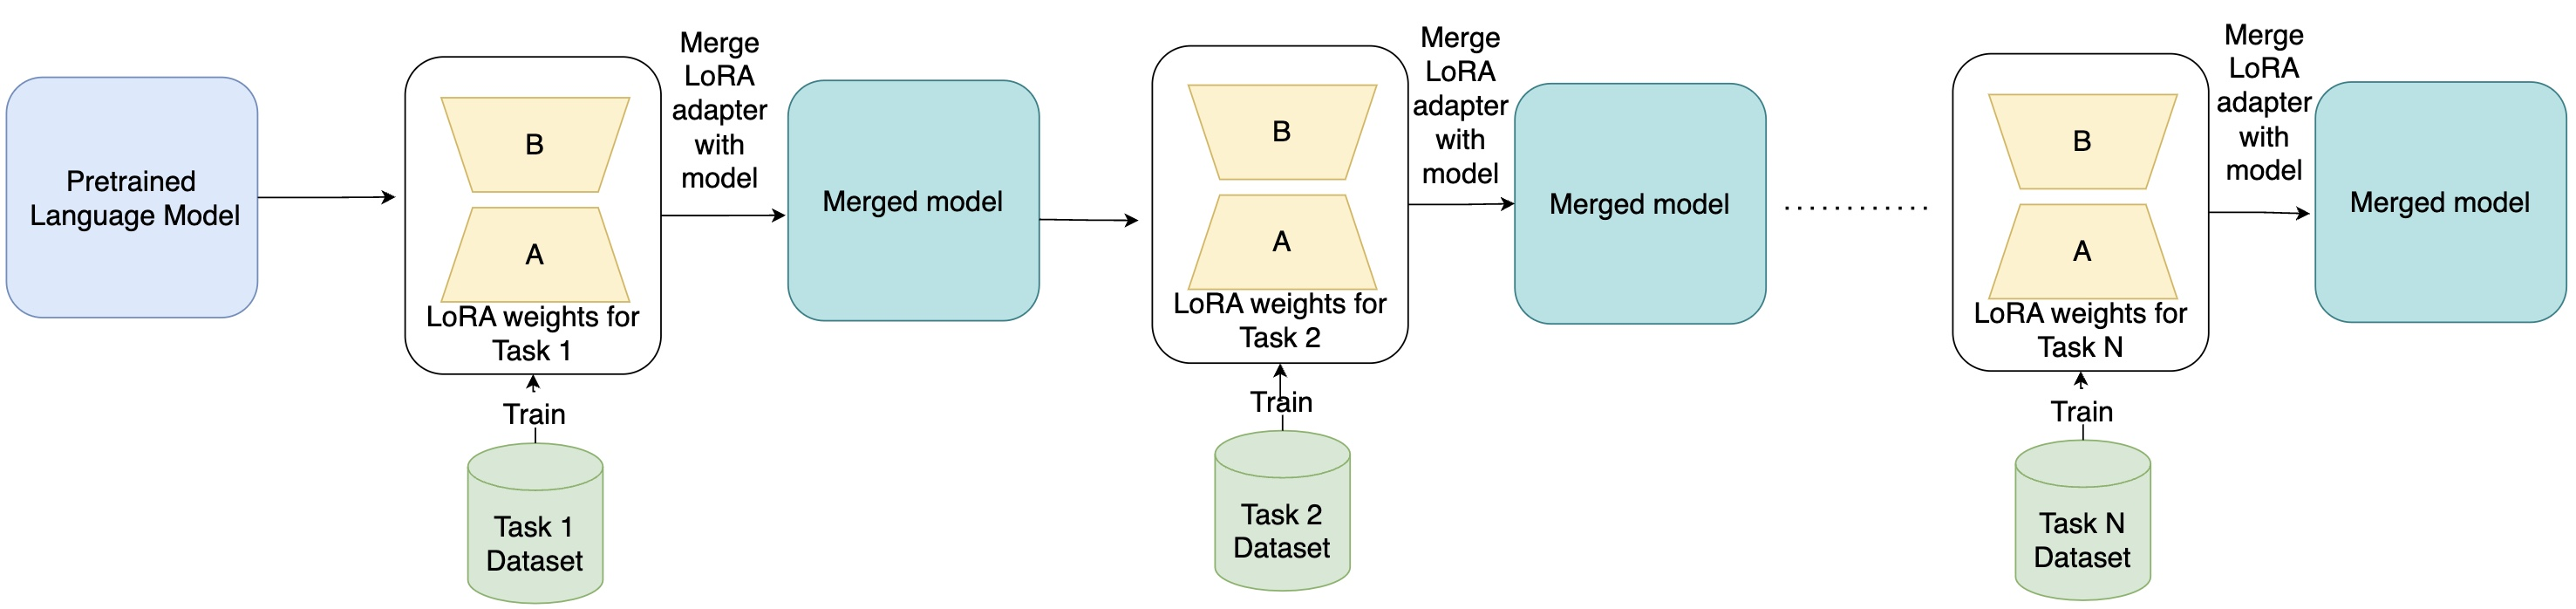
\includegraphics[width=1\textwidth]{Figures/methodology/lora_finetuning.jpeg} 
    \caption{Sequential training and merging of LoRA Adapters}
    \label{fig:SequentialTraining}
\end{figure}

The pipeline used a comprehensive evaluation with different benchmarks to track changes to the model’s pre-trained capabilities and task-specific evaluations to track model performance on tasks across fine-tunes. Our implementation used CORE replay (Section \ref{Core}) as a mitigation strategy for catastrophic forgetting. To validate the effectiveness of the mitigation approach, we implemented baseline comparisons of task-incremental learning without replay. The pipeline was constructed to address and answer the research questions posed in Section \ref{ResearchQuestions}.

\subsection{Baseline implementation} \label{baseline_setup}
The process for baseline experiments started with the step to prepare instruction data for each task. Then pre-evaluation was performed on the instruct model using different benchmarks and task-specific evaluations. Then task-specific fine-tuning was performed where a LoRA adapter was trained on the task dataset and the trained adapter was merged with the base model if the task is the 1st one in the experiment run and with the merged model from the previous fine-tune if not the 1st task. The task-specific fine-tuning and post-evaluations steps were repeated for each subsequent task.

\begin{figure}
    \centering
    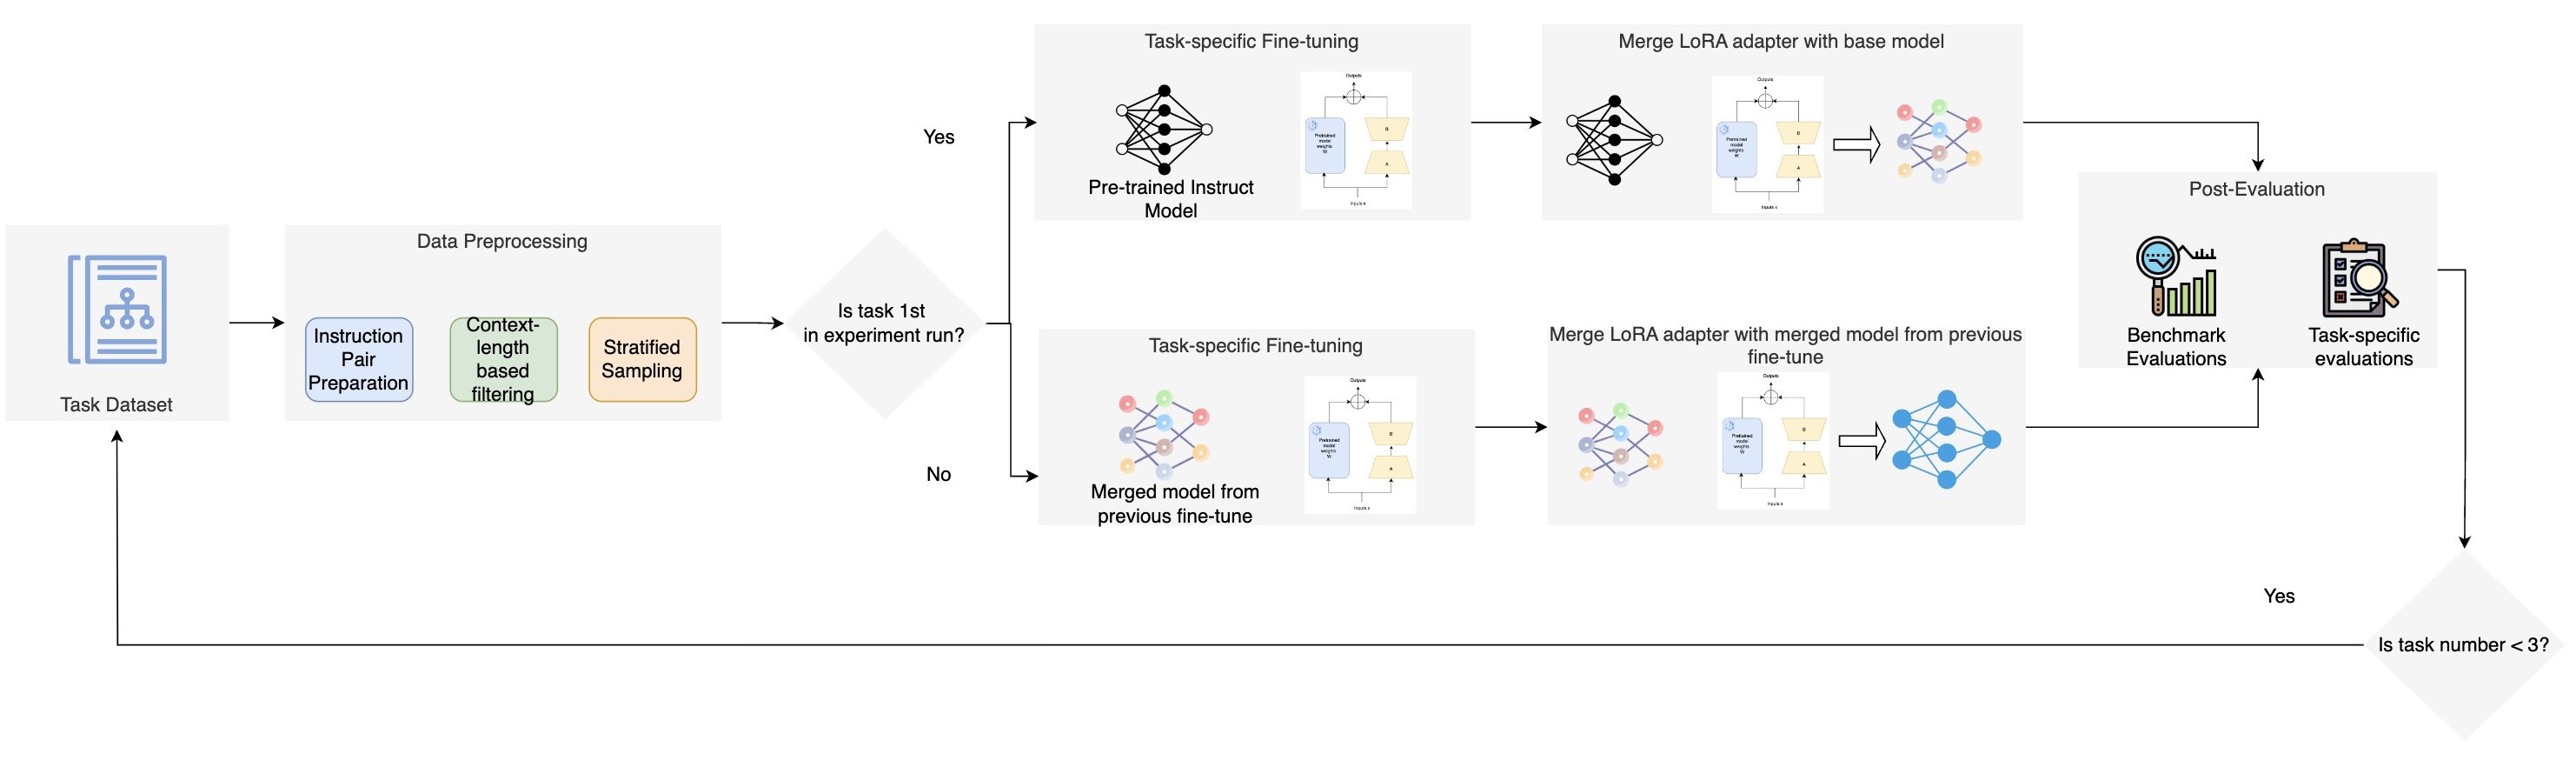
\includegraphics[angle=90, width=1.8\textheight, height=1.8\textwidth, keepaspectratio]
    {Figures/methodology/baseline_process.jpeg}
    \caption{Baseline Process Pipeline.}
    \label{fig:BaselineProcess}
\end{figure}

The task-specific fine-tuning and evaluation process are described in detail in the following sections.

\subsubsection{Task-specific fine-tuning} \label {TaskSpecificFineTuning}
The pre-trained instruct model was trained on a specific task by using Supervised Instruction Fine-tuning. The following tools were used for performing the fine-tuning: 
\begin{enumerate}
\item \href{https://huggingface.co/docs/transformers/en/index}{Transformers}: The Transformers library was used to download and use the pre-trained model.
\item \href{https://huggingface.co/docs/datasets/en/index}{Datasets}: The Datasets library was used to load the task dataset.
\item  \href{https://huggingface.co/docs/trl/en/sft_trainer}{SFT Trainer}: The SFT Trainer in the \href{https://huggingface.co/docs/trl/en/index}{Transformer Reinforcement Learning (TRL)} library from \href{https://huggingface.co/}{HuggingFace} was used for performing instruction fine-tuning on the task dataset.
\item \href{https://huggingface.co/docs/peft/en/index}{PEFT}: The PEFT library was used to perform LoRA-based parameter efficient fine-tuning. 
\item \href{https://mlflow.org/docs/latest/introduction/index.html}{MLflow}: The MLflow library was used for logging and tracking the parameters, metrics, and artifacts prepared during the model fine-tuning process.
\end{enumerate}

For performing instruction fine-tuning on a task, we first prepared the instruction dataset for the task using the steps described in Section \ref{data_preparation}. The train and validation sets for the task were used for training and evaluation in the fine-tuning process. However, we did not use a metric during the training evaluation, so loss was computed on the validation set. 
The different steps followed in the fine-tuning process were as follows:
\begin{enumerate}
\item The train and validation sets for the task were first loaded.
\item The task number was checked.
\begin{enumerate} [label*=\arabic*.]
\item If it was the 1st task in the experiment run, then the base model and the tokenizer were loaded.
\item If it was the 2nd or 3rd task in the experiment run, then the merged model and saved tokenizer from the previous fine-tune were loaded.
\end{enumerate}
\item The data collator was set up and instantiated by passing an instruction template, a response template, and the tokenizer. The instruction and response templates were based on the prompt formats used by the base model.

For Code Generation use case, the instruction template was “\#\#\# Instruction” and the response template was “\#\#\# Response”.

For Natural Language Generation use case, the instruction template was\\
<|start\_header\_id>user<|end\_header\_id|> \\
and the response template was\\
<|start\_header\_id>assistant <|end\_header\_id|>.
\item The samples from the train and validation datasets were then formatted to follow the prompt format described in Section \ref{DeepSeekPrompt} for Code Generation tasks and Section \ref{Llama3Prompt} for Natural Language Generation tasks.
\item The training parameters were set up in the form of TrainingArguments. 
\item Logging was set up to report the logs to MLFlow.
\item The configuration was set up for using LoRA adapter during fine-tuning.
\item The training arguments along with the LoRA configuration and the data collator were provided to the SFT Trainer.
\item The LoRA adapter was then trained on the task data using the SFT Trainer.
\item After the model training, the trained LoRA adapter was saved.
\item The model was merged using adapter merging (Section \ref{AdapterMerging}).
\begin{enumerate}
\item If it was the 1st task in the experiment run, the LoRA adapter was merged with the base model.
\item If it was the 2nd or 3rd task in the experiment run, the LoRA adapter was merged with the merged model from the previous fine-tune.
\end{enumerate}
\item Finally, the merged model was saved. 
\end{enumerate}


\subsubsection{Adapter merging} \label{AdapterMerging}
When using LoRA, we only train the LoRA adapter and not the full model. Thus, only the adapter weights are saved when saving the model after training. To save the full model, it is necessary to merge the adapter weights to the model weights. The merge\_and\_unload function from the PEFT library was used to do this. The merged model could then be used for inference.
\begin{figure}[h!]
    \centering
    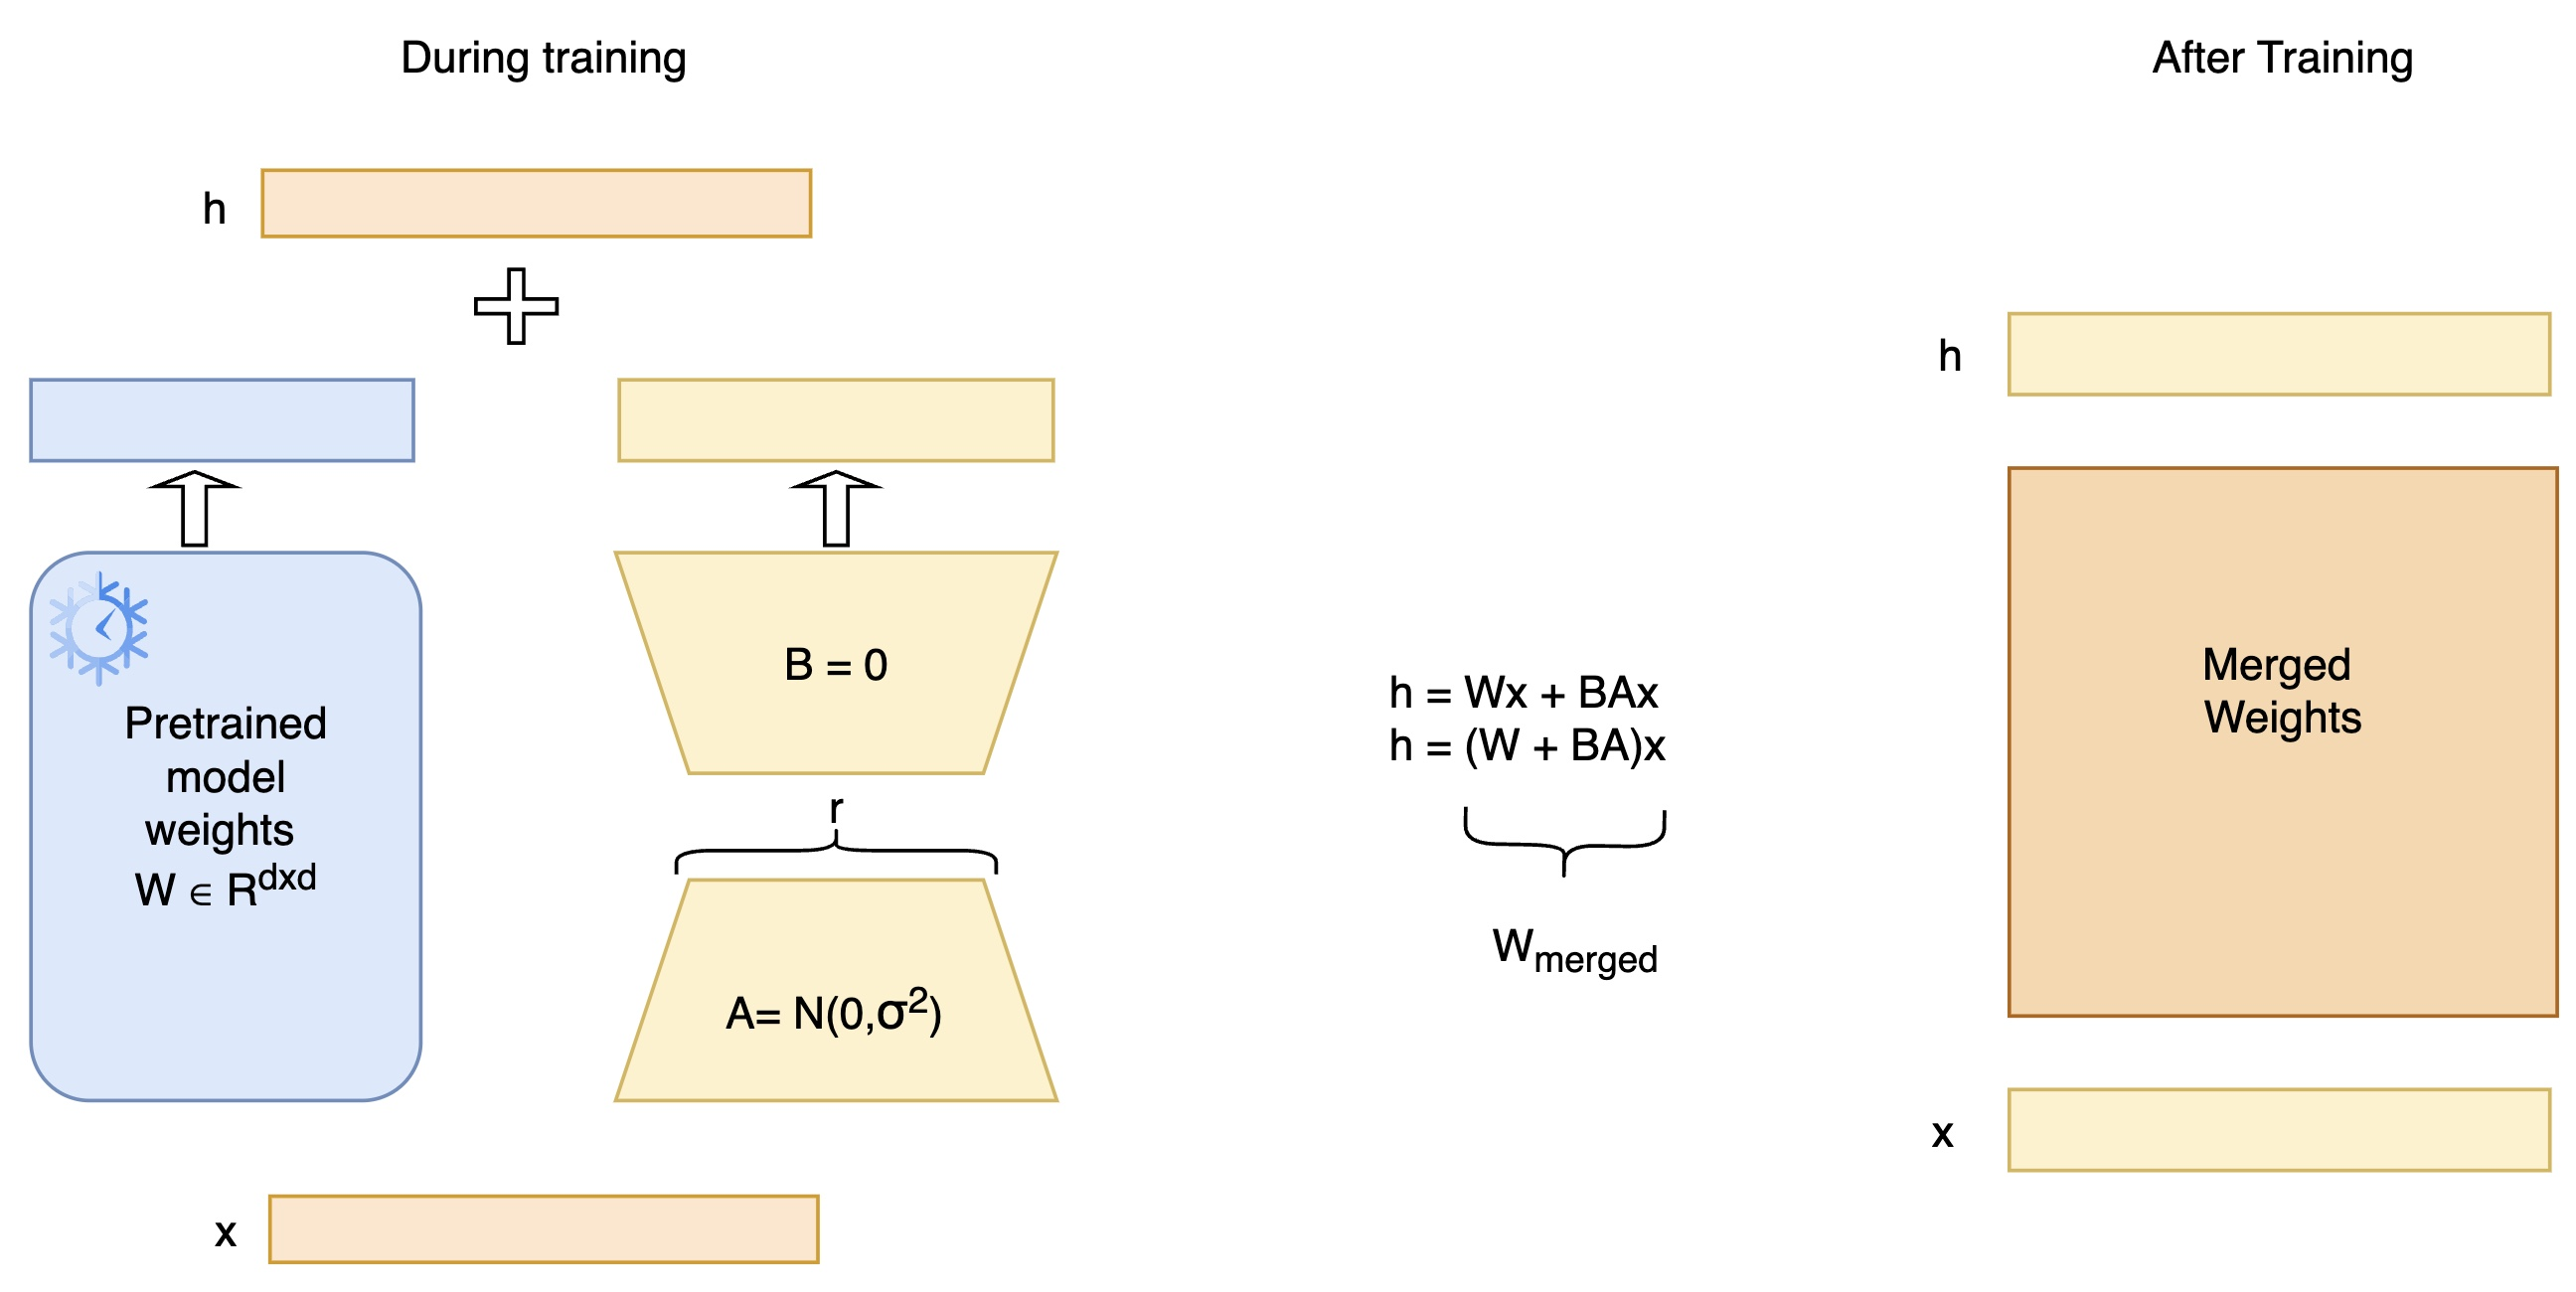
\includegraphics[width=1\textwidth]{Figures/methodology/adapter_merging.jpeg} 
    \caption{Merging LoRA adapter to base model}
    \label{fig:AdapterMerging}
\end{figure}

\subsubsection{Evaluation}
In our implementation, we used a comprehensive approach to assess the performance of the fine-tuned models across different benchmarks and task-specific evaluations. Suitable benchmarks that aligned with our use cases were selected to measure and compare the pre-trained model capabilities. Additionally, we performed task-specific evaluations where we evaluated the model on the test set and validation set of each task to measure and track the model performance before and after each fine-tuning step. This enabled us to measure the model’s ability to learn new knowledge and its capability to retain knowledge from previously learned tasks. We used task-specific performance metrics for each evaluation.
For each experiment run, the evaluation was carried out in the following stages:
\begin{enumerate}
\item Pre-evaluation: In this stage, we evaluated the base model capabilities on the benchmarks and task-specific evaluations.
\item Post-evaluation: In this stage, we evaluated the merged model capabilities on the benchmarks and task-specific evaluations after each fine-tuning step.
\end{enumerate}

\paragraph{Benchmark evaluations}
As discussed in Section \ref{benchmarks}, benchmarks are standardized frameworks for assessing an LLM’s performance. For each use case, we identified different benchmarks to measure the model’s pre-trained capabilities. The benchmark evaluation process for each use case is described as follows:
\subparagraph{Code Generation}
For Code Generation use case, we evaluated the model performance on two benchmarks: HumanEval (+ MultiPL-E) (Section \ref{humaneval}) and CoNaLa (Section \ref{conala}). 

HumanEval, originally designed for Python, and its multilingual extension, MultiPL-E are designed to evaluate the code generation abilities of the model. We used these benchmark datasets to evaluate the functional correctness of the code generated by the model in C++, Java, and Python languages. The dataset for Python is from the HumanEval benchmark and the datasets for C++ and Python are from the MultiPL-E benchmark. The pass@1 metric %(Section \ref{pass@k}) 
was used for this evaluation, which measures the proportion of correct solutions generated in the first attempt. Each sample in this dataset contained a prompt with import statements and a function declaration. Each sample also contained unit tests for the function. The task for the model was to generate code to complete the function. For C++ and Java evaluations, the gcc compiler and OpenJDK library were used at compile time. The steps taken in performing the evaluation with this benchmark were as follows:
\begin{enumerate}
\item For each sample in the dataset,
\begin{enumerate} [label*=\arabic*.]
\item The output from the model was first generated using the sample prompt.
\item The model output was cleaned to extract the generated code.
\item The unit test functions in the sample were then concatenated with the cleaned output.
\item For Java and C++, the javac and gcc compilers were used respectively to compile the complete code. For Python, the completed code was prepared for execution, since Python code does not need to be compiled.
\item The complete code was then executed and checked to see if it passed all associated unit tests. The number of samples that passed all the tests were then counted. 
\end{enumerate}
\item The pass@1 score was computed using the formula defined in Section \ref{pass@k}.
\end{enumerate}


This process was repeated for each language dataset ( C++, Java, and Python). The results from this evaluation allowed us to evaluate a model’s code generation abilities for three programming languages. The total number of samples in each language dataset is shown below:
\begin{table}[h]
\centering
\caption{Number of samples in HumanEval + MultiPL-E evalution datasets}
\begin{tabular}{{| m{3cm} | m{4cm} |}}
\hline
Language & Number of samples \\
\hline
Python & 164 \\
Java & 158 \\
C++ & 161 \\
\hline
\end{tabular}
\end{table}
We performed sample size experiments with the DeepSeek-6.7B-instruct model and used the scores reported by DeepSeek on these datasets to compare the model performance with smaller sample sizes. We were able to achieve results similar to the reported results using half the sample size. For consistency, we used 80 samples from each language dataset for the evaluation. This step was done to reduce the number of samples to conduct faster evaluations. The results from the sample size experiment are shown in Table \ref{tab:DeepSeekSampleSize}.

\begin{table}[H]
\centering
\caption{Sample size experiment performed for HumanEval (+ MultiPL-E) benchmark datasets}
\begin{tabular}{|l|l|l|l|l|ll}
\cline{1-5}
Model & Dataset & Sample Size & Score & Reported score &  &  \\ \cline{1-5}
DeepSeek-1.3B-Instruct & Python  & 164         & 0.6463                             & 0.652          &  &  \\ \cline{1-5}
DeepSeek-6.7B-Instruct & Python  & 164         & 0.7926                             & 0.786          &  &  \\ \cline{1-5}
DeepSeek-1.3B-Instruct & Python  & 80          & 0.6125                             & 0.652          &  &  \\ \cline{1-5}
DeepSeek-1.3B-Instruct & Python  & 50          & 0.6400                             & 0.652          &  &  \\ \cline{1-5}
DeepSeek-1.3B-Instruct & Python  & 40          & 0.6500                             & 0.652          &  &  \\ \cline{1-5}
DeepSeek-6.7B-Instruct & Python  & 40          & 0.7500                             & 0.786          &  &  \\ \cline{1-5}
DeepSeek-1.3B-Instruct & Java    & 158         & 0.4430                             & 0.519          &  &  \\ \cline{1-5}
DeepSeek-6.7B-Instruct & Java    & 158         & 0.6709                             & 0.684          &  &  \\ \cline{1-5}
DeepSeek-1.3B-Instruct & Java    & 80          & 0.4625                             & 0.519          &  &  \\ \cline{1-5}
DeepSeek-6.7B-Instruct & Java    & 80          & 0.6250                             & 0.684          &  &  \\ \cline{1-5}
DeepSeek-1.3B-Instruct & Java    & 40          & 0.5250                             & 0.519          &  &  \\ \cline{1-5}
DeepSeek-1.3B-Instruct & CPP     & 161         & 0.4658                             & 0.453          &  &  \\ \cline{1-5}
DeepSeek-6.7B-Instruct & CPP     & 161         & 0.6770                             & 0.634          &  &  \\ \cline{1-5}
DeepSeek-1.3B-Instruct & CPP     & 80          & 0.5000                             & 0.453          &  &  \\ \cline{1-5}
DeepSeek-6.7B-Instruct & CPP     & 80          & 0.6500                             & 0.634          &  &  \\ \cline{1-5}
DeepSeek-1.3B-Instruct & CPP     & 40          & 0.3750                             & 0.453          &  &  \\ \cline{1-5}
\end{tabular}
\label{tab:DeepSeekSampleSize}
\end{table}


CoNaLa is designed to test the model’s ability to generate code from natural language instructions. We used CodeBLEU (Section \ref{codebleu}) to evaluate the performance of the model on this benchmark. Each sample in the dataset contained intent for code generation expressed in natural language and the ground truth response for that intent. The task of the model was to generate code that satisfied the expressed intent. The steps taken to perform evaluation with the CoNaLa benchmark were as follows:
\begin{enumerate}
\item For each sample in the dataset,
\begin{enumerate} [label*=\arabic*.]
\item The output from the model was generated.
\item The model output was then cleaned to extract the generated code.
\end{enumerate}
\item The CodeBLEU score was then calculated using the formula defined in Section \ref{codebleu} by providing both the generated output and the ground truth for all samples.
\end{enumerate}

The CoNaLa benchmark dataset contained 500 samples in the test set. The sample size for the evaluation dataset was reduced to 100 to perform speedier evaluations.

\subparagraph{Natural Language Generation}
For natural language generation, we evaluated the model performance on two benchmarks: ARC-Challenge (Section \ref{arc}) and GSM8K (Section \ref{gsm8k}). 

ARC-Challenge is a subset of the ARC benchmark. We used this benchmark to evaluate the reasoning capabilities of the model. The benchmark contained multiple-choice questions. Each sample in the dataset contained a question, choices, and the answer key. The answer key is the ground-truth answer. We used Exact Match (Section \ref{accuracy}) metric for the evaluation of this benchmark. We followed the evaluation procedure used by \href{https://github.com/meta-llama/llama3/blob/main/eval\_details.md}{Llama3} for this evaluation. 
We used 25-shot examples and provided all the choices in the prompt. The prompt for this evaluation was constructed as:
\begin{lstlisting}
Question: {question}
Choices:
{choices}
{25-shot examples}
Choose the correct choice. At the end, you MUST write only the option.
\end{lstlisting}

The 25-shot examples used for this evaluation are included in the Appendix \ref{25shot}. The steps taken to perform this evaluation were:
\begin{enumerate}
\item For each sample in the dataset,
\begin{enumerate} [label*=\arabic*.]
\item The prompt was constructed in the format shown above.
\item The model output was generated using the constructed prompt.
\item The model output was cleaned by extracting only the answer choice.
\end{enumerate}
\item The exact match score was computed by using the formula defined in Section \ref{accuracy}.
\end{enumerate}
The result from this evaluation enabled us to measure the model’s language understanding and reasoning abilities. 
We conducted sample size experiment to check if we could reduce the number of samples for faster experimentation. The experiment results are shown in Table \ref{tab:ARCSampleExperiment}.

\begin{table}[H]
\centering
\caption{Sample size experiment performed for ARC-Challenge Benchmark}
\begin{tabular}{lllllll}
\cline{1-6}
\multicolumn{1}{|l|}{Evaluation   Benchmark}         & \multicolumn{1}{l|}{Sample size} & \multicolumn{1}{l|}{Batch size} & \multicolumn{1}{l|}{Time taken (s)} & \multicolumn{1}{l|}{Score}  & \multicolumn{1}{l|}{Reported   Score} &  \\ \cline{1-6}
\multicolumn{1}{|c|}{\multirow{4}{*}{ARC-Challenge}} & \multicolumn{1}{l|}{1172}        & \multicolumn{1}{l|}{8}          & \multicolumn{1}{l|}{175.68}         & \multicolumn{1}{l|}{0.7594} & \multicolumn{1}{l|}{0.786}            &  \\ \cline{2-6}
\multicolumn{1}{|c|}{}                               & \multicolumn{1}{l|}{586}         & \multicolumn{1}{l|}{8}          & \multicolumn{1}{l|}{107.81}         & \multicolumn{1}{l|}{0.7594} & \multicolumn{1}{l|}{0.786}            &  \\ \cline{2-6}
\multicolumn{1}{|c|}{}                               & \multicolumn{1}{l|}{293}         & \multicolumn{1}{l|}{8}          & \multicolumn{1}{l|}{62.21}          & \multicolumn{1}{l|}{0.7645} & \multicolumn{1}{l|}{0.786}            &  \\ \cline{2-6}
\multicolumn{1}{|c|}{}                               & \multicolumn{1}{l|}{147}         & \multicolumn{1}{l|}{8}          & \multicolumn{1}{l|}{39.70}          & \multicolumn{1}{l|}{0.7415} & \multicolumn{1}{l|}{0.786}            &  \\ \cline{1-6}
\end{tabular}
\label{tab:ARCSampleExperiment}
\end{table}

The GSM8K benchmark is designed to evaluate the math and logic capabilities of models. Each sample in the dataset contained a question and an answer. We used exact match as the metric for evaluate the model performance on this benchmark. To use exact match as a metric, we needed to compare and see whether the generated answer matched the ground truth. For this, we extracted the exact answer from the ground truth response and prepared the dataset to include the exact answer. Similar to ARC-Challenge, we followed the evaluation process used by Llama3 for this benchmark. We used an 8-shot chain-of-thought prompt and limited the maximum generation length to 512. The prompt used for each sample in this evaluation was constructed as:
\begin{lstlisting}
Question: {question}
Let's think step by step. At the end, you MUST write the answer as an integer after "####".
{8-shot examples}
\end{lstlisting}
The 8-shot examples used for this evaluation are included in the Appendix \ref{8shot}. The steps taken to perform this evaluation were:
\begin{enumerate}
\item For each sample in the dataset,
\begin{enumerate} [label*=\arabic*.]
\item The prompt was constructed in the format shown above.
\item The model output was generated using the constructed prompt.
\item The model output was cleaned by extracting only the answer after \#\#\#\#.
\end{enumerate}
\item The exact match score was computed by using the formula defined in Section \ref{accuracy}.
\end{enumerate}

The result from this evaluation enabled us to compare the math and logic capabilities of the model across fine-tunes. We used a sample size of 660 for all evaluations performed with the GSM8K benchmark. We reached that number by checking if reduced sample sizes could recreate the reported score. The sample size experiment is shown in the table below:
\begin{table}[H]
\centering
\caption{Sample size experiment performed for GSM8K Benchmark}
\begin{tabular}{lllllll}
\cline{1-6}
\multicolumn{1}{|l|}{Evaluation   Benchmark} & \multicolumn{1}{l|}{Sample size} & \multicolumn{1}{l|}{Batch size} & \multicolumn{1}{l|}{Time taken (s)} & \multicolumn{1}{l|}{Score}  & \multicolumn{1}{l|}{Reported Score} &  \\ \cline{1-6}
\multicolumn{1}{|c|}{\multirow{6}{*}{GSM8K}} & \multicolumn{1}{l|}{1319}        & \multicolumn{1}{l|}{16}         & \multicolumn{1}{l|}{1552.13}        & \multicolumn{1}{l|}{0.7900} & \multicolumn{1}{l|}{0.796}          &  \\ \cline{2-6}
\multicolumn{1}{|c|}{}                       & \multicolumn{1}{l|}{660}         & \multicolumn{1}{l|}{16}         & \multicolumn{1}{l|}{710.73}         & \multicolumn{1}{l|}{0.7970} & \multicolumn{1}{l|}{0.796}          &  \\ \cline{2-6}
\multicolumn{1}{|c|}{}                       & \multicolumn{1}{l|}{500}         & \multicolumn{1}{l|}{16}         & \multicolumn{1}{l|}{418.70}         & \multicolumn{1}{l|}{0.8200} & \multicolumn{1}{l|}{0.796}          &  \\ \cline{2-6}
\multicolumn{1}{|c|}{}                       & \multicolumn{1}{l|}{350}         & \multicolumn{1}{l|}{16}         & \multicolumn{1}{l|}{309.14}         & \multicolumn{1}{l|}{0.8086} & \multicolumn{1}{l|}{0.796}          &  \\ \cline{2-6}
\multicolumn{1}{|c|}{}                       & \multicolumn{1}{l|}{330}         & \multicolumn{1}{l|}{16}         & \multicolumn{1}{l|}{293.32}         & \multicolumn{1}{l|}{0.8091} & \multicolumn{1}{l|}{0.796}          &  \\ \cline{2-6}
\multicolumn{1}{|c|}{}                       & \multicolumn{1}{l|}{165}         & \multicolumn{1}{l|}{16}         & \multicolumn{1}{l|}{145.38}         & \multicolumn{1}{l|}{0.7697} & \multicolumn{1}{l|}{0.796}          &  \\ \cline{1-6}
\end{tabular}
\label{GSM8KSampleExperiment}
\end{table}

\paragraph{Task-specific evaluation}
Along with benchmark evaluations that assess a model’s capabilities on standardized datasets, it was also important to perform task-specific evaluations, especially in the context of task-incremental learning. Task-based evaluations allowed us to measure the model’s ability to learn a new task and its ability to retain the knowledge from previously learned tasks across fine-tunes. We performed task-specific evaluation for all the tasks selected for each use case. The task evaluation process for each use case is described as follows:

\subparagraph{Code Generation}
For code generation use case, we performed task-specific evaluations for the three tasks: Code generation in C/C++, Unit Test generation in C++, and Manifest generation (Section \ref{Code Generation Use Case}). We used the CodeBLEU metric for the evaluation. We used the test and validation sets prepared in Section \ref{traintestsplit} for each task for the task-specific evaluation. Each sample in the test and validation datasets contained an instruction, an input (only for Unit Test generation task), and a ground truth answer. 
The steps followed in the process to perform task-specific evaluation are as follows:
\begin{enumerate}
\item For each sample in the dataset,
\begin{enumerate} [label*=\arabic*.]
\item A prompt was constructed that included the instruction and if present, the input.
\item The model output was generated using the constructed prompt.
\item The model output was cleaned by extracting only the generated code.
\end{enumerate}
\item The CodeBLEU score was computed using the formula defined in Section \ref{codebleu} by providing the cleaned model outputs and the ground truth answers for all samples.
\end{enumerate}

This process was repeated for all three of the Code Generation use case tasks. One thing to note is that the \href{https://github.com/k4black/codebleu/tree/f9bfd319b2fca3d731b6e7203764f7078c6bc5f4}{CodeBLEU library} we used for computing the CodeBLEU score does not have the AST syntax tree and Data Flow for YAML code. To address this, we set the weights $\gamma$ and $\delta$ to be 0 for manifest generation task. For the other tasks, the value for all weights $\alpha$, $\beta$, $\gamma$, and $\delta$ were set to 0.25 each.

\subparagraph{Natural Language Generation}
For natural language generation use case, we performed task-specific evaluations for three tasks: Question Answering, Summarization, and Mathematical Reasoning (Section \ref{Natural Language Generation Use Case}). We used exact match metric (Section \ref{accuracy}) for the evaluation of Question Answering and Mathematical Reasoning tasks. We used ROUGE-L (Section \ref{rougel}) metric for the evaluation of the Summarization task. We used the test and validation sets prepared in Section \ref{traintestsplit} for the task-specific evaluation of each task. Each sample in the test and validation datasets contained a prompt and a ground truth answer. The steps followed in the process to perform task-specific evaluation are as follows:
\begin{enumerate}
\item For each sample in the test dataset,
\begin{enumerate} [label*=\arabic*.]
\item The model output was generated using the prompt in the sample.
\item The model output was cleaned by extracting only the exact answers for question answering and mathematical reasoning tasks, and by extracting the summary response for the summarization task.
\end{enumerate}
\item The type of current task was then checked.
\begin{enumerate} [label*=\arabic*.]
\item If the current task was the Question Answering task or the Mathematical Reasoning task, the exact match score was computed by using the formula defined in Section \ref{accuracy} by providing the cleaned model outputs and ground truth answers for all samples.
\item If the current task was summarization, then the ROUGE-L score was computed by using the formula defined in Section \ref{rougel} by providing the cleaned model outputs and ground truth answers for all samples.
\end{enumerate}
\end{enumerate}

This process was repeated for all three of the Natural Language Generation use case tasks.

Task-specific evaluations allowed us to measure and compare if the model performance on a particular task was improving or degrading after a specific fine-tune. This also enabled us to see if there was catastrophic forgetting of task-specific capabilities and helped us study how one task affects the other.


\subsection{Implementation of mitigation method: Replay} \label{mitigation_setup}
Our mitigation implementation used a rehearsal-based replay method for mitigating catastrophic forgetting. As discussed in Section \ref{Replay}, the replay method uses a memory buffer to store samples from previously learned tasks. This data is then combined with the training data for the new task and used to train the model. Adding samples from previously learned tasks ensures that the model gets a refresher on those tasks and the task-specific model capabilities are preserved. Among replay methods, we used the concepts from CORE replay (Section \ref{Core}) in our implementation. In particular, we used the Adaptive Quantity Allocation (AQA) (Section \ref{AQA}) strategy introduced by CORE for dynamically allocating the buffer space for each learned task. The CORE replay method only used data from previously learned tasks to populate the replay buffer. In contrast, our implementation included synthetic data generated using the base model in the replay buffer to help preserve the pre-trained capabilities of the model. The task-incremental learning implementation with the mitigation method is shown in Figure \ref{fig:ReplayFinetuning}.

\begin{figure}[h]
    \centering
    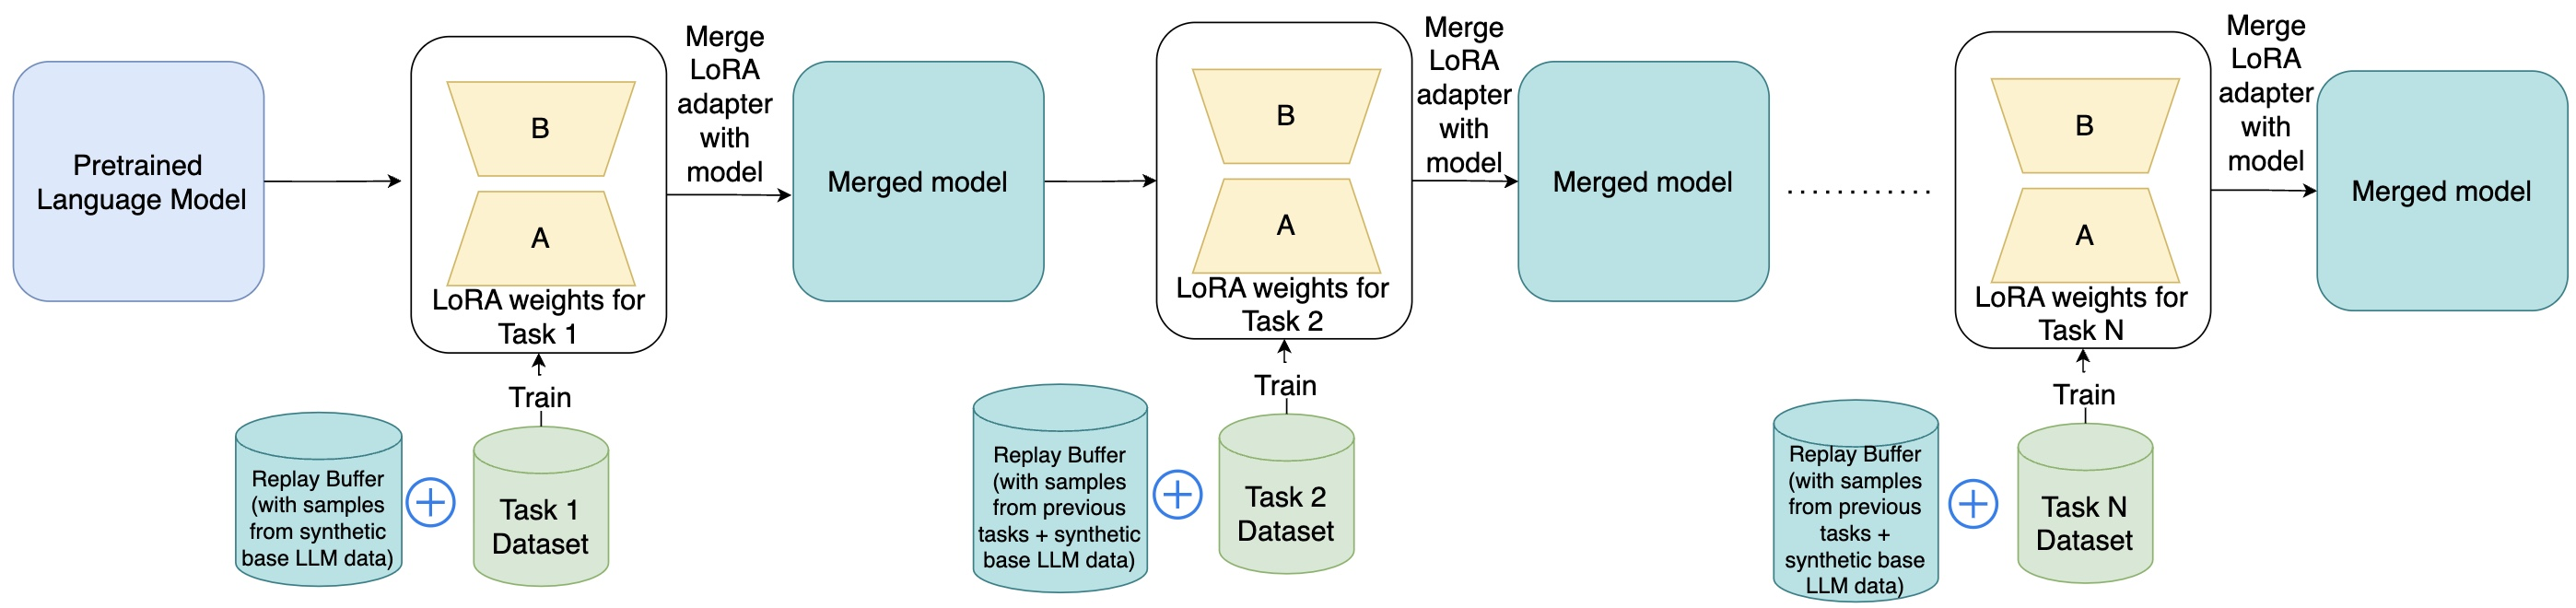
\includegraphics[width=1\textwidth]{Figures/methodology/lora_finetuning_with_replay.jpeg} 
    \caption{LoRA Fine-tuning with Replay}
    \label{fig:ReplayFinetuning}
\end{figure}

The process followed in the implementation of the mitigation method is as follows:
\begin{enumerate}
\item If the task was 1st in the experimental run, then the replay buffer was prepared by sampling from the synthetic data generated for base LLM.
\item Else, Adaptive Quantity Allocation \(AQA\) was used to dynamically allocate buffer space for each task. This was done by using the following steps:
\begin{enumerate} [label*=\arabic*.]
\item First, the forgetting rate for each completed task was computed using the formula in Section \ref{ForgettingRate}.
\item The interference rate of the current task with respect to previously learned tasks was computed using the formula in Section \ref{InterferenceRate}.
\item The attention need for the previously learned tasks was computed using the formula in Section \ref{attention}.
\item The attention need for the current task was computed using the formula in Section \ref{attention2}.
\item The attention scores were normalized for each task using softmax (Section \ref{normalized_threshold}).
\item The threshold was computed for task separation using the formula in Section \ref{threshold}.
\begin{enumerate} [label*=\roman*.]
\item If the normalized attention score was less or equal to the threshold, then the task was classified as Spaced Repetition.
\item If the normalized attention score was greater than the threshold, then the task was classified as Targeted Recall.
\end{enumerate}
\item The minimum attention score was computed for Spaced Repetition tasks using the formula in Section \ref{minimum_attention}.
\item The attention score for the Targeted Recall tasks was computed using the formula in Section \ref{TRattention}.
\item The buffer space for each task was computed based on the attention score using the formula in Section \ref{bufferspace}.
\end{enumerate}
\item Using the buffer space allocated for each task, stratified sampling was used to pick the required number of samples from the training set of previously learned tasks and the synthetically generated LLM dataset.
\item The sampled data was then combined for all previously learned tasks and synthetic LLM data.
\end{enumerate}

The data prepared for the replay buffer was added to the training dataset for the next task, and then the model was fine-tuned with the updated dataset. This ensured that the model got a refresher of the previously learned tasks, which in turn helped to mitigate catastrophic forgetting.